\documentclass[12pt]{article}

\usepackage{amsmath}
\usepackage{amssymb}
\usepackage{calc}
\usepackage{units}
\usepackage{graphicx}
\usepackage[pdftex]{hyperref}
\usepackage{subfig}
\usepackage[margin=1in]{geometry}
\usepackage{listings}
\usepackage[numbers,sort&compress]{natbib}
\usepackage{bm}
\usepackage{paralist}
\usepackage[draft]{fixme}
\usepackage{textcomp}
\usepackage{yorkdefs}

\newcommand{\halflife}{\ensuremath{T_{\nicefrac{1}{2}}}\xspace}

\hypersetup{
  breaklinks=true,
  pdftitle={Alternating Current RC Circuits},
  pdfauthor={Kevin R. Lynch based on a lab by D.C.Jain}, 
  pdfsubject={Phyiscs, Electricity and magnetism},
  pdfkeywords={resistance, capacitance, alternating current},
  pdflang={en-US},
}

\title{Alternating Current RC Circuits}
\author{}
%Kevin R. Lynch, based on an earlier lab by D.C.Jain
%\date{2012-03-07}
\date{}

\begin{document}

\maketitle

\section{Objectives}
\label{sec:objectives}

\begin{enumerate}
\item To understand the voltage/current phase behavior of RC circuits
  under applied alternating current voltages, and
\item To understand the current amplitude behavior of RC circuits
  under applied alternating current voltages.
\end{enumerate}

\section{Introduction}
\label{sec:introduction}

While we have studied the behavior of RC circuits under direct current
conditions, very few interesting circuits have purely direct currents
and constant applied voltages.  All productive or interesting circuits
operate under alternating current conditions - think computers, radios
(including cell phones), etc.  

\begin{figure}
  \centering
  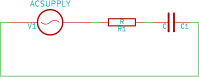
\includegraphics[width=\textwidth/2]{figures/rc-circuit}
  \caption{The RC circuit.}
  \label{fig:rccircuit}
\end{figure}
In a previous lab\footnote{\textit{The Time Constant of an RC
    Circuit}} we studied the behavior of the RC circuit under constant
applied (or DC) voltages.  Here, we will study the behavior of the
same circuit under sinusoidally alternating applied (or AC) voltages
(see Figure~\ref{fig:rccircuit}).

\section{Theory}
\label{sec:theory}

We begin analyzing this circuit the same way we analyzed the DC RC
circuit, via Kirchoff's Rules.  As before, we'll find
\begin{gather*}
  V_s(t) - V_R(t) - V_C(t) = 0\ .
\end{gather*}
Again, just as in the DC case,
\begin{align*}
  V_C(t) &= \frac{q(t)}{C} & V_R(t) &= I(t) R & I(t) =
  \deriv{q(t)}{t}\ ,
\end{align*}
leading to the differential equation
\begin{gather*}
  \deriv{q(t)}{t} + \frac{q(t)}{RC} = \frac{V_s(t)}{R}\ ,
\end{gather*}
which has the general solution
\begin{gather*}
  q(t) = e^{-t/RC} \left[ 
    q(t_0) e^{t_0/RC} + \int_{t_0}^t e^{t/RC} \frac{V_s(t)}{R} \dd t
\right]\ .
\end{gather*}
If $V_s(t)$ is allowed to be any old arbitrary function, we're stuck.
But getting stuck takes all the fun out of your work, so of course, we
won't allow it to be an arbitrary function: we'll focus on sinusoids.
This is a class of broadly useful functions - they're what come out of
the wall, they're present in electromagnetic radiation, and they are
highly amenable to mathematical manipulation and analysis.  Let's take 
\begin{gather*}
  V_s(t) = V_s \cos \omega t\ .
\end{gather*}
In Appendix~\ref{sec:solutions} we'll derive the full solution; here,
we require only the \textit{steady state response}, which gives the
time dependent charge as
\begin{gather*}
  q(t) = V_s C \frac{RC\omega}{1+(RC\omega)^2} \sin( \omega t + \phi)\ ,
\end{gather*}
where $\tan \phi = 1/RC\omega$.  We know $\phi$ as a \textit{phase
  constant}.  When we calculate the current flow, $I(t)$, in this
circuit, we find a remarkable thing:
\begin{gather*}
  I(t) = \frac{V_s}{R} \frac{(RC\omega)^2}{1+(RC\omega)^2} \cos(
  \omega t + \phi)\ .
\end{gather*}
\begin{figure}
  \centering
  \includegraphics[width=\textwidth/2]{figures/phase}
  \caption{A schematic of the phase difference between the applied
    voltage $V(t)$ and the derived current $I(t)$.}
  \label{fig:phase}
\end{figure}
Because of the presence of the capcitor, the applied voltage $V_s(t)$
gives rise to a current which not only has a frequency dependent
amplitude, but more importantly has a different phase; see
Figure~\ref{fig:phase}.  Because $phi$ is positive, the current rises
slightly before the voltage, and we say the current \textit{leads} the
voltage, or that the voltage \textit{follows} the current.  

In our teaching labs, we don't have the tools to measure the current
profile and compare it directly to the applied voltage - remember, we
only have ammeters, voltmeters, and oscilloscopes (which behave for
most purposes like voltmeters).  To use the oscilloscope to measure
this phase difference, we must find a voltage that follows exactly in
phase with the current \ldots and we have one of those: the voltage
across the resistor.  Measuring $V_R(t)$ and comparing with $V_s(t)$
allows us to measure $\phi$.
\begin{gather*}
  V_s(t) = V_s \cos \omega t\\
  V_R(t) = V_s \frac{(RC\omega)^2}{1+(RC\omega)^2} \cos( \omega t
  + \phi) = I(t) R\\
  V_C(t) = V_s \frac{RC\omega}{1+(RC\omega)^2} \sin( \omega t + \phi)\ ,
\end{gather*}

\begin{figure}
  \centering
  \subfloat[][Phases]{
    \includegraphics[width=\textwidth/3]{figures/frequency-phase}
  } \qquad
  \subfloat[][Voltage Amplitudes]{
    \includegraphics[width=\textwidth/3]{figures/frequency-amplitudes}
  }
  \caption{The phase angle as a function of angular frequency, while
    the function amplitudes are displayed on the right.  In both
    cases, the frequency is normalized in units of $1/RC$.  The phase
    is normalized to $\pi/2$, while the amplitudes are normalized to
    $V_s$.}
  \label{fig:frequency}
\end{figure}
There is one other point of interest: the behavior of the system as a
function of frequency.  Remember that our equations here account only
for the steady state behavior.  In the limit that the frequency goes
to zero (that is, we approach a DC voltage), this system should behave
just like the DC system we studied previously: $V_R(t)$ should go to
zero, and the phase difference should vanish.  You should check these
assertions; you'll find they are true.  In the other extreme, where
the frequency gets large, we have no \textit{a priori} expectations.
Plotting the behavior as a function of frequency (see
Figure~\ref{fig:frequency}), we find that the amplitude of $V_C(t)$
vanishes, while the amplitude of $V_R(t)$ goes to $V_s$, while the
phase difference between the applied voltage and resulting current
also vanishes.  In other words, the circuit acts like the capacitor
isn't even there!  Capacitors become transparent to currents at high
frequency, and opaque to currents at very low frequencies.

There is another way to view the complexities of voltages and currents
in AC RC circuits.  Note that the quantity $RC\omega$ is
dimensionless; in other words, $1/C\omega$ has the units of
resistance.  It \textit{isn't} a resistance (it's not a constant, for
starters), but it has the same units, and some of the same properties.
Let's define the quantity
\begin{gather*}
  X_C = \frac{1}{\omega C} = \frac{1}{2\pi f C}\ ,
\end{gather*}
which we'll call the \textit{capacitive reactance} of the circuit.
Next, define the \textit{impedance} $Z$
\begin{gather*}
  Z^2 = R^2 + X_C^2\ .
\end{gather*}
As it turns out, if we look only at the amplitudes of the current and
applied voltages, they are related by 
\begin{gather*}
  V_s = Z I\ ,
\end{gather*}
a sort of generalized version of Ohm's Law.  Note further that
\begin{gather*}
  \tan \phi = \frac{1}{RC\omega} = \frac{X_C}{R}\ .
\end{gather*}
Thus, $Z$ and $\phi$ can be looked on as the magnitude and direction
respectively of a \textit{vector} that gives the relative behavior of
$V_R(t)$ and $V_C(t)$ compared to $V_s(t)$.  These vectors are called
\textit{phasors}, and phasor analysis provides a useful basis for
analyzing complex AC circuits.  We will have more to say about phasors
in later labs.

\section{Procedures}
\label{sec:procedures}

\fixme{missing diagram}
\begin{figure}
  \centering
  
  \caption{The circuit under test in this lab procedure.}
  \label{fig:circuit}
\end{figure}
\fixme{missing diagram}
\begin{figure}
  \centering
  
  \caption{Definition of the points on the oscilloscope curve called
    out in Step~\ref{item:phase}.} 
  \label{fig:curvedefs}
\end{figure}
You should receive two multimeters (one of which should be a
BK-5460), an oscilloscope, a function generator, a
decade resistance box, and a decade capacitor box.

\begin{enumerate}
\item First, let's select component values for testing.  Choose a
  value for the capacitance between $\unit[0.06]{\mu F}$ and
  $\unit[0.1]{\mu F}$.  Select a frequency between \unit[300]{Hz} and
  \unit[600]{Hz}.  Calculate $X_C$ and choose a value for $R \approx
  1.2 X_C$.  Measure and record the values of $R$ and $C$
\item Configure the circuit for testing shown in
  Figure~\ref{fig:circuit}.  Use the Simpson multimeter for the
  in-circuit AC ammeter.  Record the AC current; make sure the current
  remains constant throughout the experiment.
\item Using the other meter, record the frequency $f$, and the RMS AC
  voltages across the signal generator $V_s$, $V_R$ and $V_C$.
\item \label{item:phase} Let's measure the phase shift between the
  current and applied voltage.  Make sure the two signal baselines are
  centered with respect to the horizontal and vertical axes of the
  oscilloscope, and adjust the voltage and time scales so that
  slightly more than one cycle of both waveforms is visible.  You
  should have a display that looks roughly like
  Figure~\ref{fig:curvedefs}.  We're going to record the differences
  between the zero crossings, and calculate the phase from these
  differences.  Record $A_1A_3$, $A_1B_1$, and $B_1A_2$.\fixme{These
    are wrong!}
\item Next, map out the amplitude of the current response.  Without
  changing $R$ and $C$, vary the frequency over a few points, and
  record the RMS voltage $V_s$ and RMS current $I$ at those points.
  Record you observations of the amplitudes of $V_s$ and $V_R$ on the
  oscilloscope. 
\end{enumerate}

\appendix

\section{Derivation of Solutions}
\label{sec:solutions}

which has the general solution
\begin{gather*}
  q(t) = e^{-t/RC} \left[ 
    q(t_0) e^{t_0/RC} + \int_{t_0}^t e^{t/RC} \frac{V_s(t)}{R} \dd t
\right]\ .
\end{gather*}
If $V_s(t)$ is allowed to be any old arbitrary function, we're stuck.
But getting stuck takes all the fun out of your work, so of course, we
won't allow it to be an arbitrary function: we'll focus on sinusoids.
This is a class of broadly useful functions - they're what come out of
the wall, they're present in electromagnetic radiation, and they are
highly amenable to mathematical manipulation and analysis.  Let's take 
\begin{gather*}
  V_s(t) = V_s \cos \omega t\ .
\end{gather*}
From your PHYS-151 course, you should remember that $V_s$ is the
\textit{amplitude} of the oscillation, while $\omega = 2 \pi f$ is the
\textit{angular frequency}.  With this applied voltage, we
\textit{can} perform the integration, which I leave as an exercise to
the reader.\footnote{Hint:
  \begin{gather*}
    \cos \omega t = \frac{e^{i\omega t} + e^{-i\omega t}}{2}\ .
  \end{gather*}
}
You will find\fixme{Left my notes at the office\ldots}
\begin{multline*}
  q(t) = q(t_0) e^{-(t-t_0)/RC} + \\
  C V_s \frac{RC\omega}{1+(RC\omega)^2} \sin (\omega t + \phi )\ ,
\end{multline*}

\newpage

\section*{Pre-Lab Exercises}

Answer these questions as instructed on Blackboard; make sure to
submit them before your lab session!

\begin{enumerate}
\item Ask a question
\end{enumerate}

\newpage

\section*{Post-Lab Exercises}

\begin{enumerate}
\item Discuss briefly whether you have met the objectives of the lab
  exercises.
\end{enumerate}

\end{document}

%%% Local Variables: 
%%% mode: latex
%%% TeX-master: t
%%% End: 
